\section{Introducción}

En el marco de la implementación de la Ley N.º 21.180 sobre Transformación Digital del Estado, el Departamento de Tecnologías de la Información y las Comunicaciones de la Subsecretaría para las Fuerzas Armadas ha impulsado diversas iniciativas orientadas a modernizar la gestión documental institucional. Entre ellas se encuentra DocuDigital, proyecto destinado a preservar, centralizar y facilitar el acceso a la documentación histórica proveniente de las antiguas Subsecretarías de Guerra, Marina y Aviación.

Actualmente, DocuDigital se encuentra en su segunda versión y opera como una aplicación web para la consulta y recuperación de documentos digitalizados. La plataforma dispone de mecanismos de búsqueda basados en campos descriptivos, mediante los cuales es posible localizar distintos tipos de antecedentes administrativos.

\subsection{Problema a Resolver}

DocuDigital v2 presenta limitaciones asociadas a la heterogeneidad de los procesos de digitalización utilizados por las antiguas subsecretarías. Debido a que cada organismo definió de manera independiente sus propios criterios de registro y clasificación, documentos de naturaleza equivalente pueden contener campos distintos, estructuras inconsistentes o atributos sin correspondencia directa. Esta falta de estandarización dificulta la integración de la información en un repositorio centralizado y reduce la efectividad del actual mecanismo de búsqueda.

Adicionalmente, el sistema no dispone de información detallada sobre el contenido textual de los documentos digitalizados. En general, solo se conoce la categoría documental a la que pertenece cada archivo, sin contar con una descripción precisa de los antecedentes contenidos en su interior. En consecuencia, se dificulta la identificación de documentos específicos y aumenta el tiempo requerido para localizar antecedentes relevantes para la Subsecretaría para las Fuerzas Armadas.

\subsection{Acercamiento a la Solución }

Con el propósito de abordar las limitaciones de estandarización y recuperación de información presentes en DocuDigital v2, se está desarrollando de DocuDigital v3. Esta nueva versión conserva el acceso al repositorio histórico existente e incorporará funcionalidades para el ingreso de nuevos documentos y la ejecución de búsquedas avanzadas.

Dentro de esta evolución, el presente proyecto se centra en la incorporación de un sistema de transcripción y análisis documental basado en inteligencia artificial. La solución permitirá extraer el contenido textual de los documentos digitalizados y transformarlo en información estructurada, con el fin de homogeneizar, cuando la naturaleza del documento lo permita, los campos asociados a antecedentes de una misma categoría.

A partir de la información extraída, el sistema generará metadatos y descripciones de contenido que complementarán los datos actualmente disponibles. Esto permitirá mejorar los procesos de indexación y búsqueda, reducir la dependencia de campos definidos durante los antiguos procesos de digitalización y facilitar la identificación de los antecedentes contenidos en cada documento.

Debido a las restricciones de infraestructura tecnológica de la institución, la implementación deberá priorizar herramientas libres y de código abierto que sean compatibles con el hardware disponible. Asimismo, la solución deberá hacer un uso eficiente de los recursos computacionales y permitir el procesamiento de un volumen elevado de documentos, sin comprometer la estabilidad ni la continuidad operacional del sistema.

\subsection{Estado del Arte y de la Técnica}

\subsubsection{Reconocimiento Óptico de Caracteres a la comprensión documental}

El reconocimiento óptico de caracteres (OCR, \textit{Optical Character Recognition}) tiene como propósito convertir el texto presente en una imagen en una representación digital codifica y procesable por sistemas informáticos. Aunque esta definición puede sugerir una conversión directa entre píxeles y caracteres, el reconocimiento de documentos reales requiere distinguir regiones, identificar líneas o bloques, determinar el orden de lectura y reconstruir la relación entre los elementos de una página \cite{afkari2025transformers}, como se observa en la figura \ref{fig:ocr_dg}. Esta complejidad se debe a que los documentos no contienen únicamente texto continuo, sino que pueden integrar columnas, encabezados, tablas, fórmulas, figuras, sellos y anotaciones cuya posición contribuye a su significado \cite{subramani2021document}.

\begin{figure}[H]
    \centering
    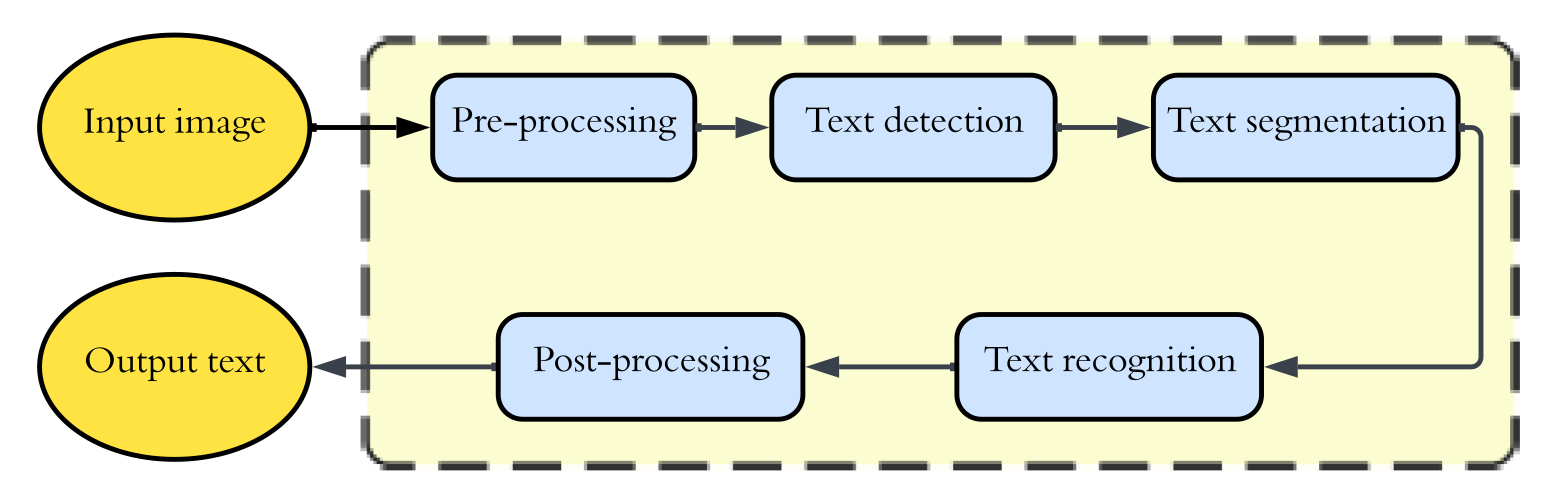
\includegraphics[width=0.5\linewidth]{images/estado del arte/ocr_diagram.png}
    \caption{Descripción general de un sistema OCR tradicional \cite{afkari2025transformers}}
    \label{fig:ocr_dg}
\end{figure}

La comprensión documental amplía el objetivo del OCR desde la transcripción hacia la recuperación conjunta del contenido y de su estructura lógica. Bajo este enfoque, una página puede transformarse en texto plano, Markdown, HTML o una representación estructurada que conserve títulos, párrafos, tablas y relaciones espaciales. Esta distinción es relevante porque una salida puede contener la mayoría de las palabras originales y, aun así, resultar poco útil si modifica el orden de lectura, mezcla columnas o destruye la organización de una tabla \cite{neudecker2021ocreval}. Por consiguiente, la calidad de un sistema documental no debe evaluarse exclusivamente por la presencia de caracteres correctos, sino también por su capacidad para preservar la forma en que la información está organizada.

El problema se vuelve más exigente en documentos escaneados, históricos o producidos bajo condiciones no controladas. El deterioro del papel, el bajo contraste, las manchas, la inclinación, las sombras y la resolución limitada alteran la apariencia de los caracteres y dificultan su separación respecto del fondo \cite{nguyen2021postocr}. Los errores generados en esta etapa se propagan hacia tareas posteriores, debido a que una fecha, un nombre o un identificador transcrito incorrectamente puede afectar la indexación, la búsqueda y la extracción automática de metadatos. En lenguas, tipografías o colecciones con pocos datos de entrenamiento, estas dificultades aumentan porque los modelos disponen de menor evidencia para representar las variaciones visuales y lingüísticas del dominio \cite{agarwal2024lowresource}.

\subsubsection{Preprocesamiento de documentos}

Antes de aplicar un modelo de reconocimiento, es posible reducir parte de la variabilidad visual mediante técnicas de preprocesamiento. Su finalidad no es modificar el contenido, sino facilitar la separación entre los trazos y el fondo para que el modelo reciba una entrada más uniforme. La ecualización adaptativa del histograma (AHE, Adaptive histogram equalization) mejora el contraste de manera local, lo que permite realzar regiones poco visibles sin aplicar la misma transformación a toda la página \cite{pizer1987ahe}. De forma complementaria, la binarización adaptativa calcula umbrales a partir del entorno de cada región y resulta apropiada cuando la iluminación o el color del fondo varían dentro del documento \cite{sauvola2000binarization}. Estas transformaciones no garantizan una mejora universal. Un aumento excesivo del contraste puede amplificar manchas, mientras que una binarización agresiva puede eliminar trazos finos, signos de puntuación o bordes de tablas. Por esta razón, la imagen original y cada perfil de preprocesamiento deben tratarse como configuraciones experimentales independientes, en lugar de asumir que una técnica es óptima para todas las páginas.

\subsubsection{Transformadores y Modelos Visión-Lenguaje}

Los sistemas OCR basados en aprendizaje profundo evolucionaron desde arquitecturas que combinaban redes convolucionales para extraer rasgos visuales y redes recurrentes para reconocer secuencias, hacia modelos fundamentados en transformadores. El mecanismo de autoatención de estas arquitecturas permite relacionar regiones distantes de una misma entrada y representar dependencias globales, lo que resulta útil cuando una línea, una columna o una celda debe interpretarse en función de otras zonas del documento \cite{afkari2025transformers}. Esta evolución también favoreció modelos generativos capaces de producir secuencias completas en lugar de clasificar caracteres de manera aislada.

Uno de estas arquitecturas es CRNN base-atention, la cual, combina la extracción de características visuales de una CNN, el modelado secuencial de una RNN y el cálculo de pesos contextuales de la atención para procesar datos complejos con alta precisión. En la figura \ref{fig:arch_trans} se observa un diagrama de su arquitectura. 

\begin{figure}[H]
    \centering
    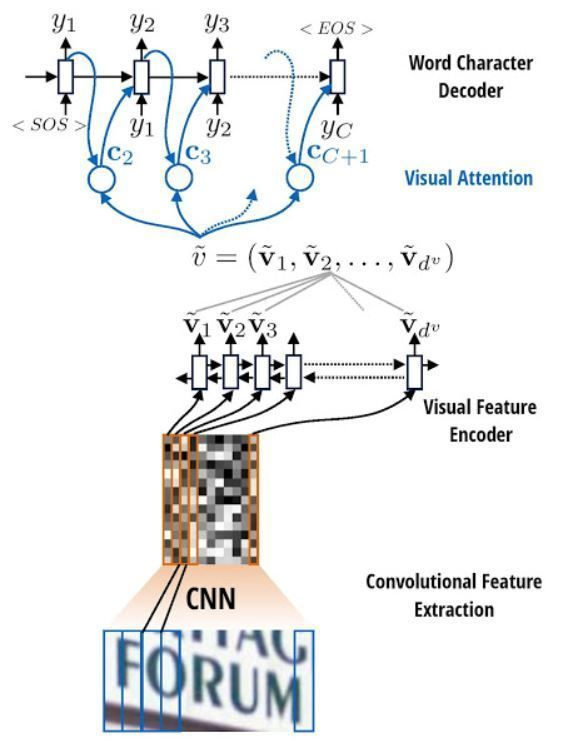
\includegraphics[width=0.4\linewidth]{images/estado del arte/arch_transformer.png}
    \caption{La arquitectura de un modelo CRNN base-attention \cite{afkari2025transformers}}
    \label{fig:arch_trans}
\end{figure}

Los modelos visión-lenguaje (VLM, \textit{Vision-Language Models}) integran representaciones visuales y lingüísticas dentro de una misma arquitectura. De manera general, un componente visual transforma la imagen en representaciones internas, un mecanismo de proyección las vincula con el espacio lingüístico y un modelo de lenguaje genera la respuesta condicionada por la imagen y por las instrucciones proporcionadas \cite{zhang2024vlmsurvey}, como se observa en la figura \ref{fig:vlm_ejem}. Aplicados a documentos, estos modelos pueden recibir una página completa y generar una secuencia que combine transcripción, orden de lectura y marcado estructural, reduciendo la necesidad de conectar manualmente múltiples módulos especializados.


\begin{figure}[H]
    \centering
    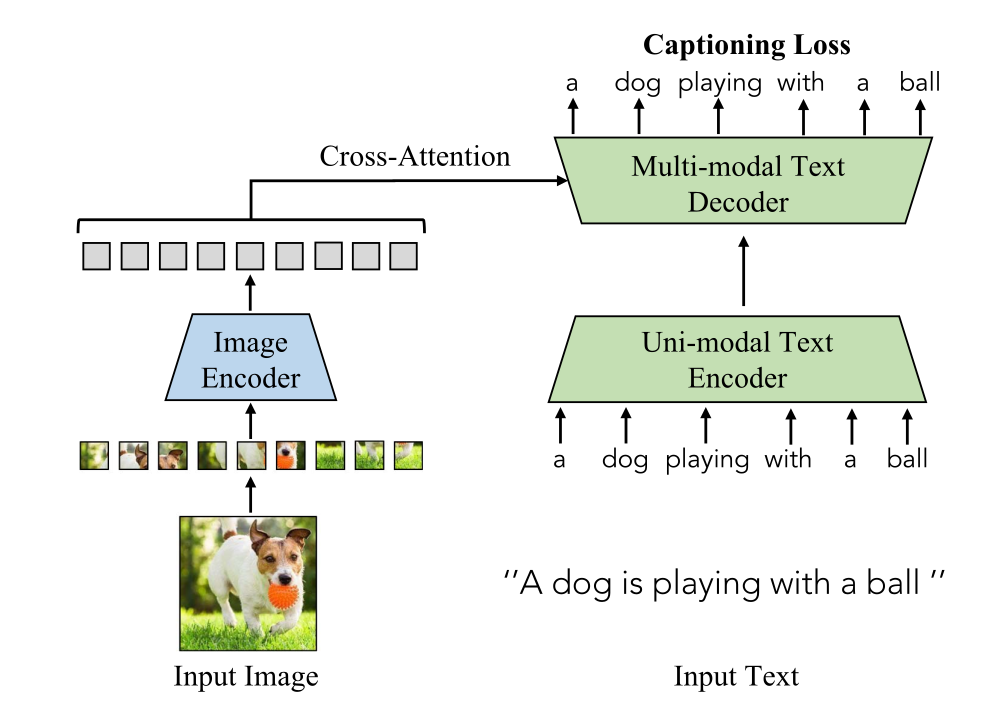
\includegraphics[width=0.5\linewidth]{images/estado del arte/vlm_ejem.png}
    \caption{Ilustración simplificada de la generación de COCA image-to-caption \cite{zhang2024vlmsurvey}}
    \label{fig:vlm_ejem}
\end{figure}

La principal ventaja de este enfoque es su flexibilidad, ya que un mismo modelo puede adaptarse mediante instrucciones a tareas de transcripción, descripción, extracción o conversión estructurada. Sin embargo, la generación lingüística también puede producir información plausible que no se encuentra respaldada por la imagen, fenómeno conocido como alucinación multimodal \cite{liu2024hallucination}. En consecuencia, una salida gramaticalmente correcta no constituye por sí sola evidencia de fidelidad documental. La validación debe realizarse mediante referencias verificadas y métricas que permitan detectar sustituciones, omisiones, contenido agregado y alteraciones estructurales.

\subsubsection{Modelos utilizados para el análisis documental}

Los modelos seleccionados representan distintas aproximaciones al análisis documental mediante inteligencia artificial. Para facilitar su comparación, se agrupan en dos familias: modelos visión-lenguaje de propósito general y modelos especializados en OCR y análisis documental. Esta clasificación permite relacionar la arquitectura de cada modelo con su nivel de especialización, tamaño y capacidad para procesar documentos multilingües.

\paragraph{Modelos visión-lenguaje de propósito general.}

Los modelos de la familia Qwen-VL fueron desarrollados para resolver tareas multimodales generales, entre las que se incluyen reconocimiento textual, comprensión de imágenes, análisis de documentos y razonamiento visual. \textbf{Qwen2-VL} introdujo un mecanismo de resolución dinámica que transforma imágenes de diferentes dimensiones en una cantidad variable de tokens visuales, evitando la necesidad de redimensionar todas las entradas a una resolución fija. Sobre esta base, Qwen2.5-VL-3B emplea aproximadamente 3 mil millones de parámetros y combina un codificador visual con un modelo de lenguaje autorregresivo, incorporando mecanismos de posicionamiento espacial que permiten conservar la relación entre texto, objetos y regiones de la imagen. La familia posee capacidades multilingües e incluye el procesamiento de texto en español, aunque su precisión documental depende de la calidad visual, la estructura de la página y la representación del idioma en los datos de entrenamiento \cite{wang2024qwen2vl}.

\begin{figure}[H]
    \centering
    \includegraphics[width=0.8\linewidth]{images/estado del arte/qwen3-vl.png}
    \caption{Arquitectura del modelo Qwen3-VL \cite{bai2025qwen3vl}.}
    \label{fig:qwen3-vl}
\end{figure}

\textbf{Qwen3-VL} amplía esta arquitectura mediante el mecanismo DeepStack, que incorpora al modelo de lenguaje características procedentes de diferentes niveles del codificador visual. Esta integración permite combinar detalles visuales locales con representaciones semánticas de mayor nivel. Asimismo, utiliza una variante mejorada de MRoPE para representar conjuntamente las dimensiones espaciales y secuenciales de la entrada. En este proyecto se considera la variante Qwen3-VL-2B, compuesta por aproximadamente 2 mil millones de parámetros. El modelo presenta capacidades multilingües para reconocimiento y comprensión visual, incluyendo el español; sin embargo, al tratarse de un VLM de propósito general, su rendimiento en transcripción y reconstrucción documental debe verificarse mediante una evaluación específica sobre los documentos de interés \cite{bai2025qwen3vl}.


La principal ventaja de esta familia reside en su versatilidad, dado que un mismo modelo puede reconocer texto, interpretar elementos visuales y responder instrucciones sobre el contenido. No obstante, esta generalidad implica un mayor espacio de tareas y no garantiza que la transcripción documental alcance el mismo nivel de precisión que un modelo entrenado específicamente para OCR.

\paragraph{Modelos especializados en OCR y análisis documental.}

A diferencia de los VLM de propósito general, los modelos especializados concentran su entrenamiento y arquitectura en la extracción de texto, la recuperación del orden de lectura y la representación de elementos estructurales, como tablas, fórmulas, gráficos y sellos.

\begin{figure}[H]
    \centering
    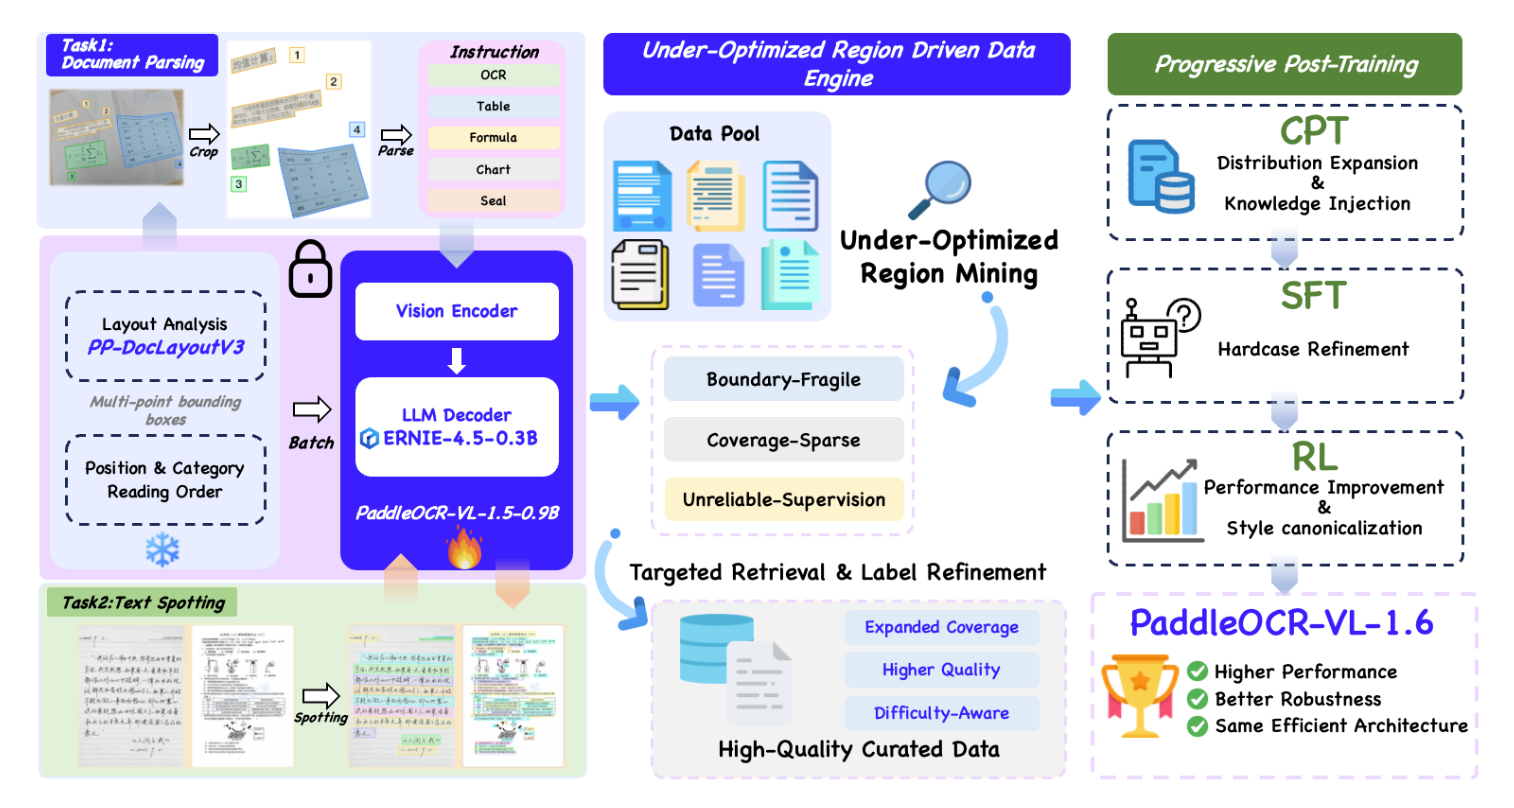
\includegraphics[width=0.7\linewidth]{images/estado del arte/paddle.png}
    \caption{Visión general del \textit{pipeline} PaddleOCR-VL-1.6 \cite{zhang2026paddleocrvl}.}
    \label{fig:paddle}
\end{figure}

\textbf{PaddleOCR-VL-1.6 }utiliza un \textit{pipeline} de dos etapas, como se observa en la figura \ref{fig:paddle}. En la primera, PP-Doc\allowbreak LayoutV3 analiza la distribución de la página y localiza sus regiones mediante cajas delimitadoras multipunto, lo que permite tratar documentos con perspectiva, curvatura o diseños irregulares. En la segunda etapa, cada región es procesada por PaddleOCR-VL\allowbreak-1.6-0.9B, un modelo de aproximadamente 0,9 mil millones de parámetros que integra un codificador visual de resolución nativa, un conector MLP adaptativo y el modelo lingüístico ERNIE-4.5-\allowbreak0.3B. El modelo reconoce texto, tablas, fórmulas, gráficos y sellos, mientras que un módulo de posprocesamiento reorganiza las predicciones en formatos como Markdown o JSON. La familia PaddleOCR-VL admite 109 idiomas e incluye explícitamente el español, por lo que posee soporte directo para documentos escritos en este idioma \cite{zhang2026paddleocrvl}.


\begin{figure}[H]
    \centering
    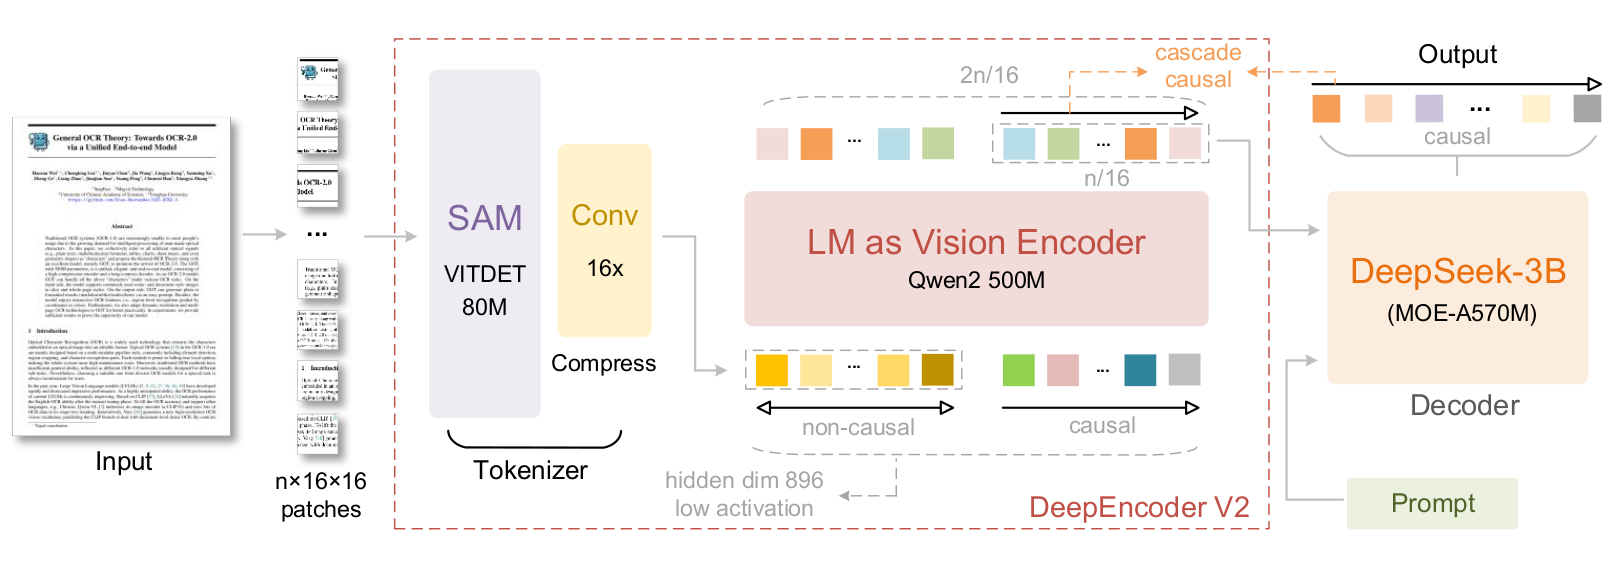
\includegraphics[width=0.7\linewidth]{images/estado del arte/deepseek-ocr2.png}
    \caption{Arquitectura del modelo DeepSeek-OCR 2 \cite{wei2026deepseekocr2}.}
    \label{fig:deepseek}
\end{figure}

\textbf{DeepSeek-OCR 2} emplea una arquitectura codificador--decodificador orientada a modelar el orden semántico de los documentos. Su componente DeepEncoder V2 combina un codificador visual compacto, atención bidireccional y consultas causales que reorganizan los tokens visuales antes de entregarlos al modelo de lenguaje. De esta manera, el procesamiento no queda restringido a un recorrido espacial fijo de izquierda a derecha y de arriba hacia abajo, sino que puede adaptarse a la estructura lógica de la página. Las representaciones obtenidas se entregan a un decodificador DeepSeek de 3 mil millones de parámetros con arquitectura \textit{Mixture-of-Experts}, encargado de generar autorregresivamente la transcripción o representación estructurada \cite{wei2026deepseekocr2}. El modelo se describe como multilingüe.

\begin{figure}[H]
    \centering
    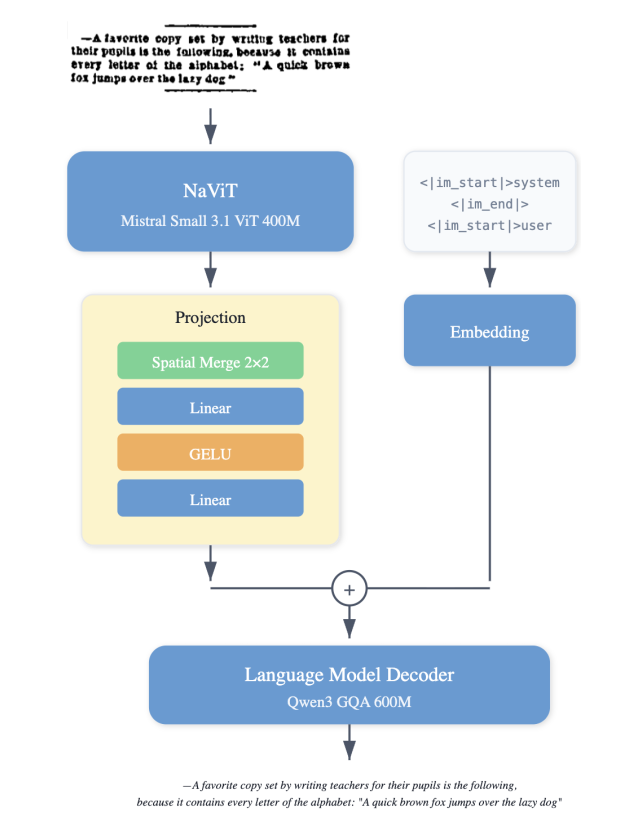
\includegraphics[width=0.5\linewidth]{images/estado del arte/lightOnOcr.png}
    \caption{Arquitectura del modelo LightOnOCR-2-1B \cite{taghadouini2026lightonocr}.}
    \label{fig:light}
\end{figure}

\textbf{LightOnOCR-2-1B }adopta un enfoque completamente \textit{end-to-end}, mediante el cual una página documental se transforma directamente en una secuencia textual estructurada sin ejecutar módulos independientes de detección, reconocimiento y reconstrucción del orden de lectura. El modelo posee aproximadamente 1.000 millones de parámetros y combina un codificador visual de resolución nativa inicializado desde Mistral-Small-3.1, un proyector multimodal que reduce en cuatro veces el número de tokens visuales mediante agrupación espacial, y un decodificador Qwen3 que genera la transcripción de forma autorregresiva. Su entrenamiento prioriza documentos escaneados, publicaciones científicas y lenguas europeas, con especial énfasis en francés. Por esta razón, el modelo dispone de capacidad para procesar texto en español por su base multilingüe y su cobertura de lenguas europeas \cite{taghadouini2026lightonocr}.

\begin{figure}[H]
    \centering
    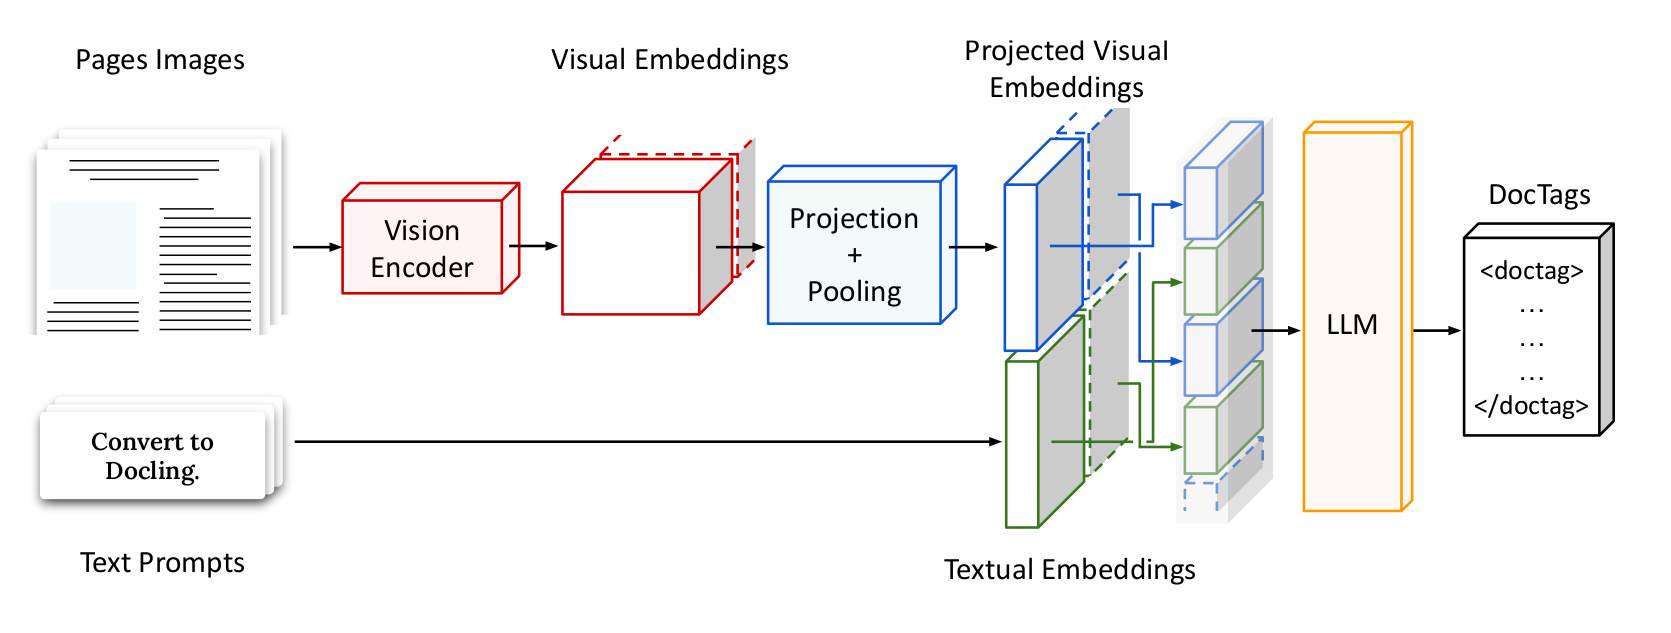
\includegraphics[width=0.5\linewidth]{images/estado del arte/docling.png}
    \caption{Arquitectura del modelo SmolDocling \cite{nassar2025smoldocling}.}
    \label{fig:docling}
\end{figure}

\textbf{Granite-Docling-258M} es un modelo visión-lenguaje \textit{end-to-end} de aproximadamente 258 millones de parámetros, especializado en convertir imágenes documentales en representaciones estructuradas mediante DocTags. Su arquitectura, que se observa en la figura \ref{fig:docling},se basa en IDEFICS3 e integra un codificador visual SigLIP2-base-patch16-512, encargado de extraer las características de la página, con un modelo de lenguaje Granite de 165 millones de parámetros que genera autorregresivamente el contenido, la estructura y la ubicación de elementos como texto, tablas, fórmulas, listas, código e imágenes. IBM lo describe como un modelo multilingüe \cite{ibm2025granitedoclingannouncement}.



En síntesis, los modelos analizados reflejan dos estrategias complementarias para el procesamiento documental. Los VLM de propósito general, representados por la familia Qwen-VL, ofrecen mayor flexibilidad para combinar reconocimiento textual, comprensión visual y razonamiento multimodal, mientras que los modelos especializados concentran su diseño en la extracción fiel del contenido, la recuperación del orden de lectura y la reconstrucción de elementos estructurales. Dentro de esta segunda familia, PaddleOCR-VL adopta un \textit{pipeline} por etapas, DeepSeek-OCR 2 reorganiza las representaciones visuales según la estructura semántica de la página, LightOnOCR realiza una conversión generativa completamente \textit{end-to-end} y Granite-Docling produce una representación compacta basada en DocTags. Por tanto, no existe una arquitectura universalmente superior, ya que la elección depende del equilibrio requerido entre precisión, conservación estructural, capacidad multilingüe, consumo de recursos y robustez frente a documentos complejos o degradados.


\subsubsection{Cuantización y ejecución en infraestructura local}

El uso local de modelos multimodales está condicionado por la memoria disponible y por la capacidad de cómputo del equipo. La cuantización reduce estos requerimientos al representar pesos o activaciones con menos bits que los utilizados durante el entrenamiento \cite{gholami2021quantization}. Esta reducción disminuye el tamaño del modelo y el tráfico de memoria, pero introduce una aproximación numérica que puede afectar la calidad de la salida. La degradación no es necesariamente gradual ni equivalente entre tareas, debido a que determinadas capas o distribuciones de valores son más sensibles a la reducción de precisión \cite{jin2024quantization}.

En OCR, la cuantización debe analizarse con especial cuidado porque diferencias pequeñas pueden modificar cifras, fechas, nombres propios o delimitadores estructurales. Por ello, el ahorro de memoria no puede considerarse suficiente para validar una configuración; debe relacionarse con métricas de fidelidad obtenidas sobre documentos representativos. Herramientas como \texttt{llama.cpp} permiten ejecutar modelos cuantizados en CPU, GPU o esquemas híbridos, facilitando su despliegue sobre hardware de propósito general \cite{sparrenberg2025llamacpp}. No obstante, el rendimiento efectivo depende del formato cuantizado, los kernels disponibles, la arquitectura del procesador, la aceleración por tarjeta de video y la distribución de la carga entre memoria y cómputo.


\subsubsection{Benchmarking y reproducibilidad experimental}

La comparación entre modelos requiere un benchmark que mantenga constantes los factores externos a la solución evaluada. Esto implica utilizar los mismos documentos, perfiles de preprocesamiento, parámetros de generación, condiciones de hardware y reglas de medición. Los marcos de evaluación de inferencia destacan que los resultados solo son comparables cuando la carga de trabajo y el procedimiento se encuentran definidos de manera explícita \cite{reddi2020mlperf}. Asimismo, cada ejecución debe conservar identificadores que permitan relacionar el documento, la página, el modelo, la cuantización, el perfil visual y la salida obtenida.

Bajo restricciones de hardware, el mejor modelo no es necesariamente aquel que obtiene la mayor precisión en una única métrica. Una configuración puede ser inviable si excede la memoria disponible, presenta tiempos de respuesta incompatibles con la operación o genera resultados inestables. Por tanto, la selección debe considerar simultáneamente fidelidad, latencia, consumo y robustez, manteniendo trazabilidad suficiente para reproducir cada comparación. Este criterio convierte el benchmark en un instrumento de decisión técnica y no únicamente en una clasificación de modelos.

\subsubsection{Evaluación de la fidelidad textual y estructural}

La evaluación combina métricas textuales, secuenciales y estructurales, debido a que los errores del análisis documental pueden manifestarse como caracteres sustituidos, palabras omitidas, contenido añadido, alteraciones del orden de lectura o reconstrucciones incorrectas de tablas. Antes de calcular los indicadores, la referencia y la predicción se someten al mismo proceso de normalización. Este procedimiento elimina etiquetas y tokens propios de cada modelo, transforma el contenido en texto plano, decodifica entidades, unifica mayúsculas y minúsculas, compacta espacios y aplica una tokenización común. De esta forma, las métricas textuales se concentran en la fidelidad del contenido y no en diferencias superficiales de formato.

La tasa de error de caracteres, o \textit{Character Error Rate} (CER), y la tasa de error de palabras, o \textit{Word Error Rate} (WER), cuantifican la distancia de edición entre la predicción y la referencia. Ambas consideran las sustituciones, eliminaciones e inserciones necesarias para transformar una secuencia en la otra, pero operan a diferente granularidad \cite{santos2019ocreval}:

\begin{equation}
    \mathrm{CER}
    =
    \frac{S_c+D_c+I_c}{N_c},
    \qquad
    \mathrm{WER}
    =
    \frac{S_w+D_w+I_w}{N_w},
    \label{eq:cer_wer}
\end{equation}

donde $S$, $D$ e $I$ corresponden a sustituciones, eliminaciones e inserciones, mientras que $N$ representa la longitud de la referencia. CER permite identificar alteraciones finas en fechas, cifras, identificadores y nombres propios, mientras que WER refleja el efecto de los errores sobre unidades léxicas completas. En ambos casos, un valor menor indica una transcripción más fiel. A partir de estas tasas se calculan además la exactitud de caracteres y la exactitud de palabras:

\begin{equation}
    \mathrm{Acc}_{c}=\max(0,1-\mathrm{CER}),
    \qquad
    \mathrm{Acc}_{w}=\max(0,1-\mathrm{WER}).
    \label{eq:character_word_accuracy}
\end{equation}

Estas exactitudes facilitan la interpretación y visualización de los resultados, ya que un valor mayor representa un mejor desempeño. Sin embargo, la aplicación de una cota inferior igual a cero oculta la magnitud de tasas de error superiores a uno; por esta razón, CER y WER se conservan como indicadores principales del error.

La precisión, la exhaustividad y la medida $F_1$ a nivel de tokens complementan las métricas de edición al distinguir entre contenido añadido y contenido omitido. Sea $C$ la intersección multiconjunto entre los tokens de la referencia y los de la predicción, de manera que se respeten las apariciones repetidas. Estas métricas se definen como \cite{powers2011evaluation}:

\begin{equation}
    P_{\mathrm{tok}}
    =
    \frac{|C|}{|\mathrm{Pred}|},
    \qquad
    R_{\mathrm{tok}}
    =
    \frac{|C|}{|\mathrm{GT}|},
    \qquad
    F_{1,\mathrm{tok}}
    =
    \frac{2P_{\mathrm{tok}}R_{\mathrm{tok}}}
         {P_{\mathrm{tok}}+R_{\mathrm{tok}}}.
    \label{eq:token_metrics}
\end{equation}

La precisión de tokens penaliza la sobregeneración, puesto que disminuye cuando la predicción contiene fragmentos que no están respaldados por la referencia. La exhaustividad penaliza las omisiones, mientras que $F_1$ proporciona un equilibrio entre ambas dimensiones. 

%Junto con estas métricas se registran los conteos \texttt{common\_tokens}, \texttt{extra\_tokens} y \texttt{missing\_tokens}, que representan, respectivamente, la cantidad de tokens coincidentes, añadidos y omitidos. Estos valores no constituyen métricas normalizadas independientes, sino indicadores diagnósticos que deben interpretarse junto con \texttt{gt\_token\_count} y \texttt{pred\_token\_count}.

La conservación del orden de lectura se evalúa mediante una adaptación de la subsecuencia común más larga, o \textit{Longest Common Subsequence} (LCS). Esta técnica permite determinar cuántos tokens de la referencia aparecen en la predicción manteniendo su orden relativo, aunque no se encuentren de forma contigua \cite{lin2004lcs}:

\begin{equation}
    \mathrm{RO}_{\mathrm{LCS}}
    =
    \frac{\operatorname{LCS}(\mathrm{GT},\mathrm{Pred})}{|\mathrm{GT}|}
    \label{eq:reading_order_lcs}
\end{equation}

Un valor igual a uno indica que todos los tokens de la referencia aparecen en el mismo orden relativo. 

%En este proyecto, LCS se emplea como un indicador diagnóstico del orden de lectura y no como una métrica OCR estandarizada. Además, debido a que no penaliza directamente todas las inserciones, debe analizarse en conjunto con la precisión de tokens y el conteo de tokens adicionales.

La evaluación de tablas requiere considerar tanto el contenido textual como las relaciones estructurales entre filas, columnas y celdas combinadas. 

%Para ello, se deben registrar \texttt{gt\_table\_count} y \texttt{pred\_table\_count}, correspondientes al número de tablas detectadas en la referencia y en la predicción. Estos conteos permiten identificar tablas omitidas o generadas incorrectamente antes de examinar su calidad individual.

La métrica \textit{Tree-Edit-Distance-based Similarity} (TEDS) compara las representaciones HTML de dos tablas como estructuras arbóreas. La medida considera las etiquetas de los nodos, las propiedades \texttt{rowspan} y \texttt{colspan}, y el contenido de las celdas \cite{zhong2020teds}:

\begin{equation}
    \mathrm{TEDS}
    =
    \max\left(
        0,
        1-
        \frac{
            \operatorname{TED}(T_{\mathrm{Pred}},T_{\mathrm{GT}})
        }{
            \max\left(
                |T_{\mathrm{Pred}}|,
                |T_{\mathrm{GT}}|
            \right)
        }
    \right).
    \label{eq:teds}
\end{equation}

TEDS entrega un valor entre cero y uno, donde un resultado mayor representa una mayor similitud conjunta de estructura y contenido. Su utilización permite penalizar errores que no son visibles mediante una comparación lineal del texto, como celdas desplazadas, combinaciones incorrectas o desalineaciones entre filas y columnas.

La evaluación tabular se complementa con las variantes \textit{GriTS Top} y \textit{GriTS Con}, pertenecientes al marco \textit{Grid Table Similarity} \cite{smock2023grits}. GriTS representa cada tabla como una matriz y alinea sus subestructuras mediante el problema de las subestructuras bidimensionales más similares. \textit{GriTS Top} evalúa la topología de la tabla, considerando la disposición de filas, columnas y expansiones de celdas, mientras que \textit{GriTS Con} mide la similitud del contenido textual de las celdas después de establecer su correspondencia estructural. Esta separación permite determinar si una predicción falla por reconstruir incorrectamente la grilla o por reconocer de manera deficiente el contenido de las celdas.

En conjunto, CER y WER evalúan la fidelidad de la transcripción; la precisión, la exhaustividad y $F_1$ distinguen entre contenido agregado y omitido; LCS examina la conservación del orden de lectura; y TEDS, GriTS Top y GriTS Con evalúan la reconstrucción tabular desde perspectivas complementarias. Por tanto, el desempeño de los modelos no se determina mediante un único indicador, sino mediante el análisis conjunto de sus errores textuales, secuenciales y estructurales.
